%D�finir le format du document: papier, taille de police, type de document, etc.
\documentclass[a4paper, 11pt]{article}

%%%%%%%%% Packages externes utilis�s %%%%%%%%%%%%%%%%%%%
\usepackage[french]{babel}
\usepackage[latin1]{inputenc}
\usepackage[T1]{fontenc}
\usepackage{verbatim}
\usepackage{graphicx}
\usepackage{epstopdf}
\usepackage{macro}
\usepackage{algorithm}
\usepackage{algorithmic}
%\usepackage{algorithm2e}


%La mise en page du rapport, NE PAS MODIFIER.
\usepackage{geometry}
 \geometry{
 a4paper,
 left=20mm,
 right=20mm,
 top=20mm,
 bottom=20mm,
 }

%%%%%%%%% Le corps du document entre begin et end %%%%%%%%%%%%%%%%%%%
\begin{document}

%Page de garde
%%%%%%%%%%%%%%% Page de garde %%%%%%%%%%%%%%%%%%%

\begin{titlepage}{
    \begin{center}
        \vspace* {25mm}
        {\Large \textbf {Universit� de Cergy-Pontoise}} \\
        \vspace* {10mm}
        {\Large \textbf {RAPPORT}} \\
        \vspace* {10mm}
        pour le projet d'architecture des ordinateurs \\
        \textbf {Licence d'Informatique deuxi�me ann�e} \\
        \vspace* {10mm}

	sur le sujet \\
        \vspace* {10mm}
	{\Huge \textsf{Conception d'un processeur 4 bits}} \\
        \vspace* {10mm}
 	r�dig� par \\
        \vspace* {10mm}
        {\Large \textbf {GERARD Quentin et PETITEVILLE Valentin}} \\
				\vspace* {10mm}
				\noreffig{img/proc.jpg}{12.82cm}{8.2cm} \\
        \date Mai 2017
        \vspace* {10mm}
	\end{center}
}
\end{titlepage}


%G�n�ration automatique de la table des mati�res, de la liste des figures et de la liste des tableaux
\tableofcontents
\listoffigures
\listoftables

%Une section "remerciements" pourrait �tre int�ressante. C'est une section non num�rot� (avec un * )
\section*{Remerciements}
Les auteurs du projet voudraient remercier E.Ansermin, M.Belkaid et J.Lorandel.

\newpage
\section{Introduction}
\label{sec:introduction}

%Il n'y a pas d'espace au d�but du paragraphe.
\paragraph{}Dans le cadre du module de d'architecture des ordinateurs du second Semestre de L2, les �tudiants doivent r�aliser en bin�me un projet avec le logiciel Logisim en r�utilisant les �l�ments appris en cours. Le projet consiste en la r�alisation d'un processeur 4 bits.
Notre bin�me est compos� de Valentin PETITEVILLE, �tudiant en L2-I dans le groupe A, et de Quentin GERARD �tudiant en L2 CMI SIC.

\section{Sp�cification du processeur}
\label{sec:specification}

\subsection{L'ALU}
\label{sec:spec1}

\paragraph{Premier paragraphe} On commence � expliquer...

\paragraph{} Juste un simple paragraphe.

\subsection{Le banc de registre}
\label{sec:spec2}

\paragraph{} 

\subsection{L'unit� d'adressage}
\label{sec:spec3}

\paragraph{} 

\subsection{L'unit� de contr�le}
\label{sec:spec4}

\paragraph{} 
\newpage
\section{R�alisation }
\label{sec:impl}

\subsection{L'ALU}
\label{sec:real1}

\paragraph{Composition}Notre ALU est donc compos� de :
\begin{itemize}
\item 2 Entr�es sur 4 Bits
\item 1 Sortie sur 4 Bits
\item 8 Op�rations (Dont un Full Adder)
\item 1 Multiplexeur 4Bits, 8 vers 1 
\end{itemize}

\paragraph{}Voici le tableau des instructions de l'ALU:
\begin{table}[H]
\centering
\begin{tabular}{|l|l|}
\bf Op�ration & \bf Code d'Op�ration \\
\hline
ADD & 000 \\
OR & 001 \\
AND & 010 \\
NOT & 011 \\
SUBSTRACT & 100 \\
NOR & 101 \\
NAND & 110 \\
NXOR & 111 \\
\end{tabular}
\caption{Code op�ration de l'ALU}
\label{tab:alucode}
\end{table}


\begin{figure}[H]
	\centering
		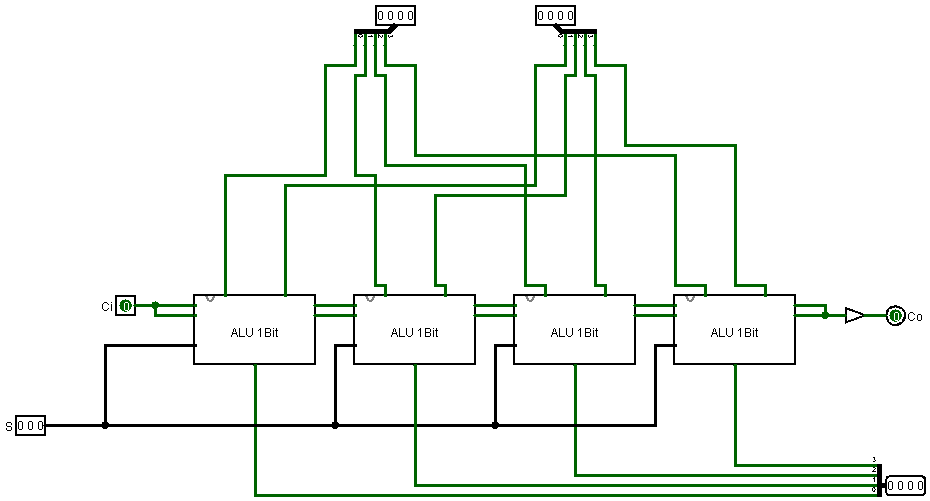
\includegraphics[width=0.75\textwidth]{./img/ALU_PROC.png}
		\caption{Sch�ma complet de l'ALU}
	\label{fig:alu}
\end{figure}

\begin{figure}[H]
	\centering
		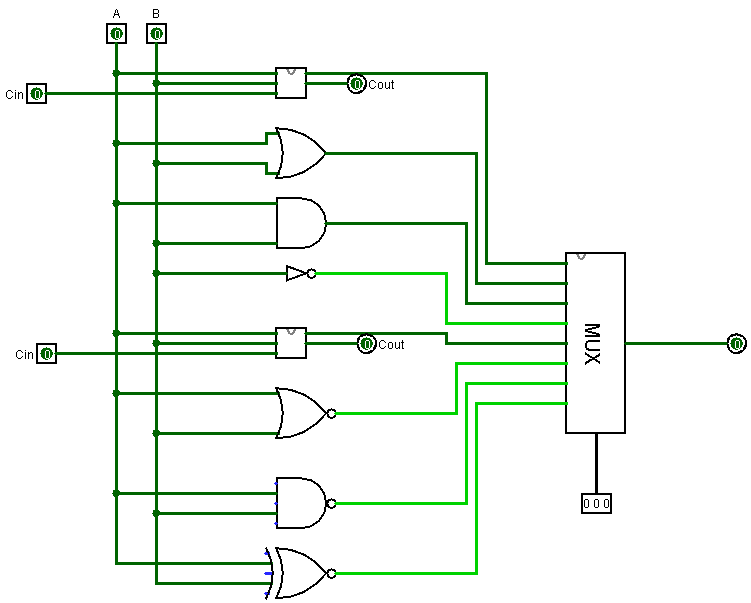
\includegraphics[width=0.75\textwidth]{./img/ALU.png}
		\caption{Sch�ma d'un ALU 1bit}
	\label{fig:mux}
\end{figure}

\begin{figure}[H]
	\centering
		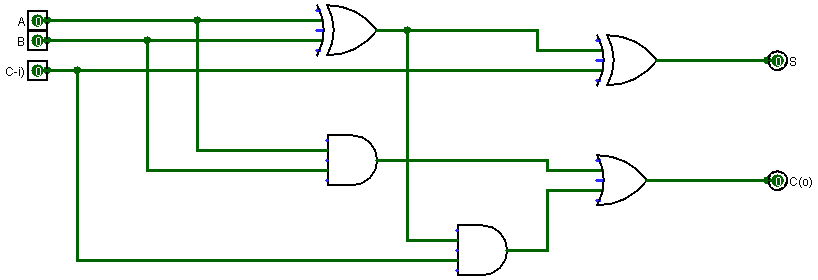
\includegraphics[width=0.75\textwidth]{./img/fulladder.png}
		\caption{Sch�ma du FullAdder}
	\label{fig:fulladder}
\end{figure}

\begin{figure}[H]
	\centering
		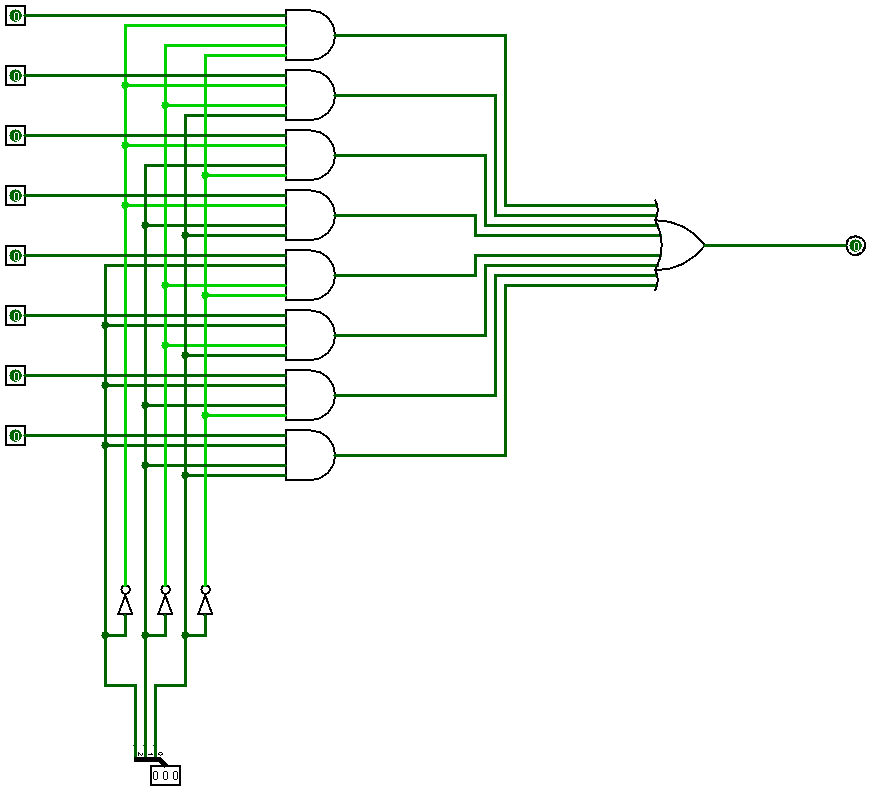
\includegraphics[width=0.75\textwidth]{./img/MUX.png}
		\caption{Sch�ma du Multiplexeur}
	\label{fig:mux}
\end{figure}

\subsection{Le banc de registre}
\label{sec:real2}

\paragraph{} Notre banc de registre est compos� de:
\begin{itemize}
\item Une entr�e 4 bits
\item 2 sorties 4 bits
\item Un decodeur sur 2 bits en entr�e
\item Un bit de validation pour l'�criture
\item 4 registres 4 bits
\item 2 s�lecteurs de registre (un pour le BUS X et l'autre pour le BUS Y)
\end{itemize}

\paragraph{Probl�me rencontr�}La bascule D que nous avons concu (grace aux sch�ma du cours), cr�ait des probl�me d'oscillation lors du fonctionnement du registre, nous avons donc utilis� les registres implement� dans Logisim pour notre registre 4 bit. Nous avons pr�fer� utilis� les registres de Logisim plutot que de remplac� les Bascule D par des D Latch, malgr� que ces derniers fonctionnait tr�s bien, car nous voulions profiter des avantages que nous offrait l'utilisation de l'horloge native � Logisim, notamment l'insensibilit� au changement du signal entre deux front d'horloge, et ainsi anticiper un eventuel futur disfonctionnement du banc de registre.

\begin{figure}[H]
	\centering
		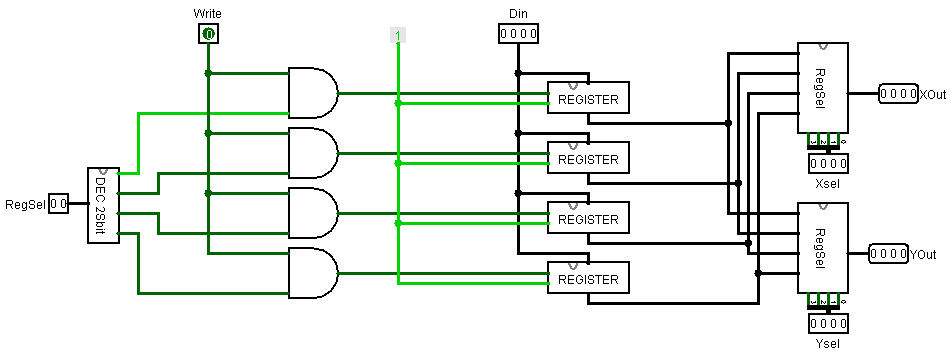
\includegraphics[width=0.75\textwidth]{./img/REGFILE.png}
		\caption{Sch�ma du banc de registres}
	\label{fig:REGFILE}
\end{figure}

\begin{figure}[H]
	\centering
		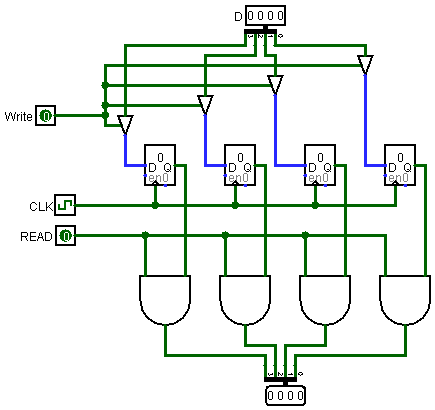
\includegraphics[width=0.75\textwidth]{./img/REG4bits.png}
		\caption{Sch�ma d'un registre 4bits}
	\label{fig:REG 4 bits}
\end{figure}

\begin{figure}[H]
	\centering
		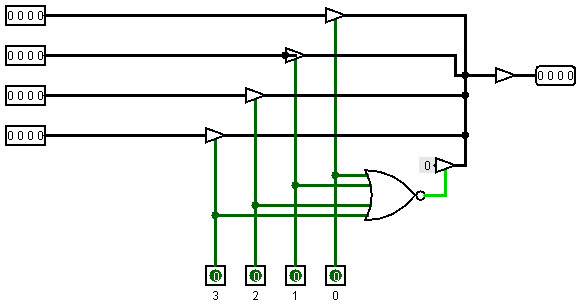
\includegraphics[width=0.75\textwidth]{./img/REGSEL.png}
		\caption{Sch�ma du s�lecteur de registre}
	\label{fig:REGSEL}
\end{figure}

\subsection{L'Unit� d'adressage}
\label{sec:real3}
\paragraph{}Notre Unit� d'adressage est compos� de 2 parties:
\begin{itemize}
\item Partie Instructions:
\begin{itemize}
\item 1 entr�e 4bits (Adresse de la prochaine instructions)
\item 2 sorties 4bits (Adresse de l'instruction en cours; Une sortie pour la m�moire d'instruction; Une sortie pour l'Unit� de controle destin� au calcul de l'adresse de la prochaine instruction)
\item Un registre d'adresse 4bits
\item Un bit de validation d'�criture
\end{itemize}
\item Partie Donn�es
\begin{itemize}
\item 1 entr�e 4bits
\item 1 sortie 4bits 
\item 1 bit de validation d'�criture dans la m�moire de donn�es
\end{itemize}
\end{itemize}

\paragraph{Probl�me rencontr�}Nous pouvons remarquer que la partie g�rant la m�moire de donn�es ne contient pas de registre d'adresse, en effet nous n'avons pas compris le r�le de ce registre, et son implementation provoque un disfonctionnement dans notre processeur du au retard provoqu� sur l'arriv� de l'information � la m�moire RAM.

\begin{figure}[H]
	\centering
		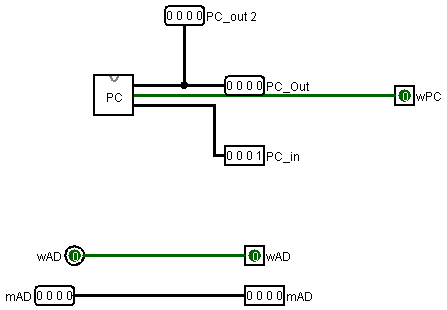
\includegraphics[width=10cm,height=6cm]{./img/UA.png}
		\caption{Sch�ma complet de l'Unit� d'adressage}
	\label{fig:UA}
\end{figure}

\begin{figure}[H]
	\centering
		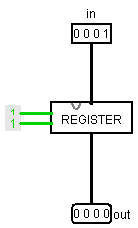
\includegraphics[width=4cm,height=6cm]{./img/PC.png}
		\caption{Sch�ma du registre d'adresse d'instruction (PC)}
	\label{fig:PC}
\end{figure}

\subsection{L'unit� de contr�le}
\label{sec:real4}

\paragraph{} Notre unit� de contr�le est compos�e d'un registre d'instruction ainsi que de multiple d�codeur d'instruction, s'occupant chacun d'une partie de l'instruction, et de plusieurs selecteurs de sorties.

\paragraph{Probl�me rencontr�} Bien que nous l'ayons impl�ment�, la sortie Fetch nous � pos� probl�me, en effet nous ne comprenons son r�le dans le processeur, c'est pourquoi la sortie est tout de m�me branch� � une constante (elle doit visiblement �tre constament � 1) mais pas utilis�.

\begin{figure}[H]
	\centering
		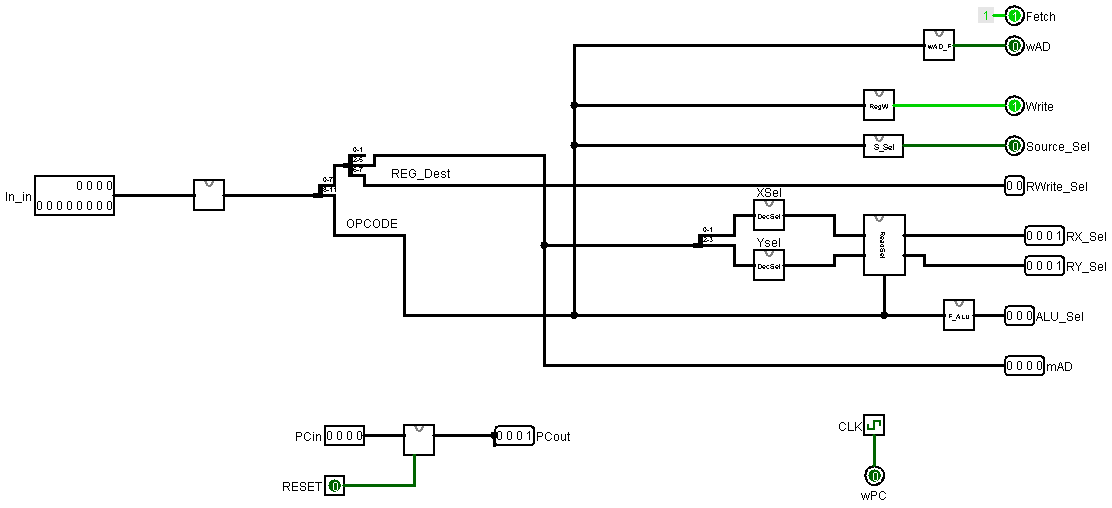
\includegraphics[width=0.75\textwidth]{./img/UC.png}
		\caption{Sch�ma complet de l'Unit� de contr�le}
	\label{fig:UC}
\end{figure}

\begin{figure}[H]
	\centering
		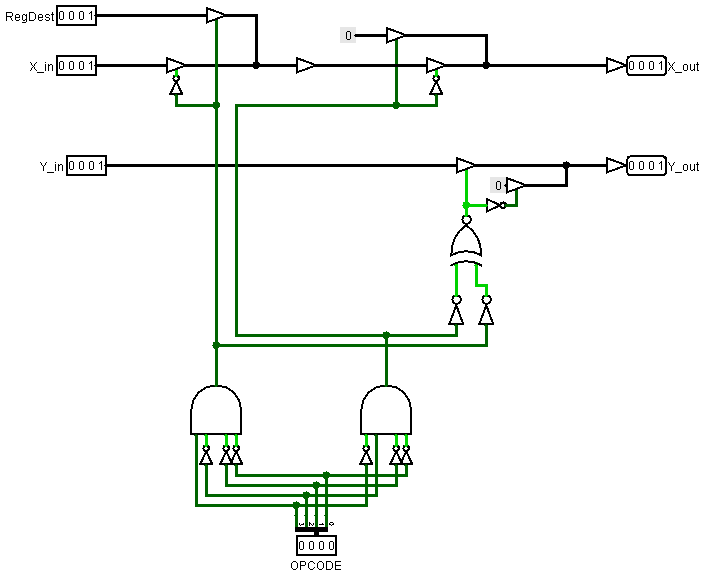
\includegraphics[width=0.75\textwidth]{./img/ReadSelector.png}
		\caption{Sch�ma complet du s�lecteur de lecture}
	\label{fig:ReadSelector}
\end{figure}

\subsection{Le CPU}
\label{sec:real5}
\paragraph{}Enfin notre CPU relie tous les composants vu ci dessus, ainsi que la m�moire RAM servant de m�moire de donn�es ainsi qu'une m�moire ROM contenant le programme du processeur (la m�moire d'instruction).

\paragraph{}Voici le tableau des instructions du processeur:
\begin{table}[H]
\centering
\begin{tabular}{|l|l|}
\bf Op�ration & \bf Code d'Op�ration \\
\hline
ADD & 0000 \\
OR & 0001 \\
AND & 0010 \\
NOT & 0011 \\
SUBSTRACT & 0101 \\
LOAD & 0100 \\
STORE & 1000 \\
\end{tabular}
\caption{Code op�ration du CPU}
\label{tab:opcode}
\end{table}


\begin{figure}[H]
	\centering
		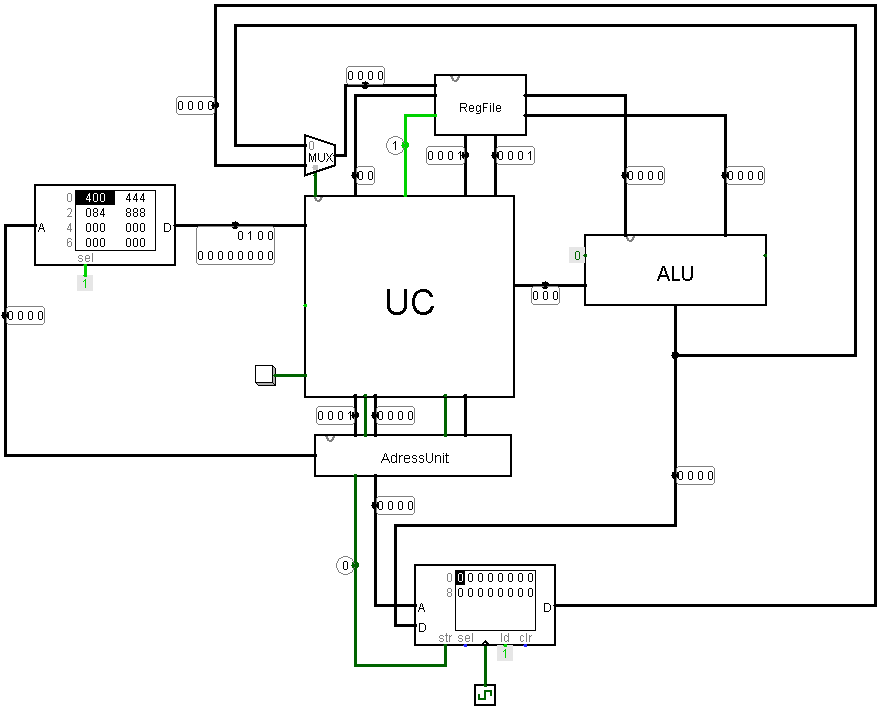
\includegraphics[width=0.75\textwidth]{./img/CPU.png}
		\caption{Sch�ma complet du processeur}
	\label{fig:CPU}
\end{figure}

\newpage
\section{Extension}
\label{sec:ext}

\subsubsection{La soustraction}
\label{sec:ext1}

\paragraph{} Par manque de temps nous n'avons pas pu integrer la soustraction a notre ALU car cela demandait de revoir l'interface de notre ALU et de l'unit� de controle. Malgr� le fait qu'elle ne soit pas int�gr�e, elle fonctionne tout de m�me.
\newpage
\section{D�roulement du projet}
\label{sec:deroulement}

\noindent Dans cette section, nous d�crivons comment la r�alisation du projet s'est d�roul�e au sein de l'�quipe de projet. 

\subsection{Synchronisation du travail}
\label{sec:synchro}

\paragraph{}Afin de pouvoir travailler sur ce projet nous avons utilis� la plateforme Github.

\subsection{R�partition du travail}
\label{sec:repartition}

\begin{table}[H]
\centering
\begin{tabular} {|p{7cm}|p{7cm}|}
\hline{\centering}
\bf Valentin & \bf Quentin \\
\hline
ALU & Banc de Registre \\
\hline
Extension & Unit� de Controle \\
\hline
Compte rendu & Unit� d'Adressage\\
\hline
\end{tabular}
\caption{R�partition des t�ches}
\label{tab:repartition}
\end{table}

\subsection{Probl�mes rencontr�s}
\label{sec:problemes}
\begin{itemize}
\item L'impl�mentation de l'op�ration soustraction
\item R�alisation de l'unit� d'adressage
\item La compr�hension de l'utilit� d'un registre d'adresse de donn�es
\item La compr�hension de certains signaux de sorties de l'UC (Fetch)
\item La bascule D qui cr�ait un probl�me d'oscillation (Nous avons donc utilis� les registres fourni par Logisim)
\end{itemize}

\end{document}
